%% Variational inference in coupled models of amino acid substitution
%% Molecular Biology and Evolution -- Methods manuscript, initial submission.
%%
%% HAND-MAINTAINED.  First produced from
%%   ../../neurips-stody-paper/paper2-coupled/neurips_workshop_paper2.tex
%% by port-from-neurips.py, which is kept as a record of that port.  Since then
%% this file has diverged (the lumpability material, cut from the NeurIPS
%% version for space, is restored here), so edit this file directly.  Re-running
%% the port script would throw those edits away.
%%
%% Formatting follows the "Manuscript formatting" section of the MBE author
%% guidelines: one PDF carrying main text, references, tables, figures and
%% captions; line numbers; double spacing; ~25 mm margins.  There is no
%% separate supplementary file -- the former appendix is a subsection of
%% Materials and Methods.

\documentclass[11pt]{article}

\usepackage[letterpaper,margin=25mm]{geometry}
\usepackage[utf8]{inputenc}
\usepackage[T1]{fontenc}

%% MBE cites by author and year, so natbib runs in author-year mode with the
%% comma between author and year suppressed: "(Cohn et al. 2010)".
\usepackage[round,authoryear]{natbib}
\setcitestyle{aysep={}}

\usepackage{setspace}
\usepackage{amsmath,amssymb,amsfonts,bm}
\usepackage{graphicx}
\usepackage{booktabs}
\usepackage{makecell}
\usepackage{tikz}
\usetikzlibrary{arrows.meta}
\usepackage{array}
\usepackage{longtable}
\usepackage{nicefrac}
\usepackage{microtype}
\usepackage{xcolor}
\usepackage{soul}       % \hl for post-submission revisions
\sethlcolor{yellow}
\newcommand{\revised}[1]{\hl{#1}}   % inserted text
% deleted text: struck through on a highlight (soul cannot nest \st in \hl,
% so the highlight is a zero-padding \colorbox; deletions must be short)
\newcommand{\deleted}[1]{{\setlength{\fboxsep}{0pt}\colorbox{yellow}{\vphantom{(}\st{#1}}}}
\usepackage{url}
\usepackage[hidelinks]{hyperref}
\usepackage[mathlines]{lineno}
\usepackage{cleveref}   % must be loaded after hyperref

%% lineno does not number displayed equations unless the amsmath environments
%% are wrapped in linenomath.  This is the standard patch.
\newcommand*\patchAmsMathEnvironmentForLineno[1]{%
  \expandafter\let\csname old#1\expandafter\endcsname\csname #1\endcsname
  \expandafter\let\csname oldend#1\expandafter\endcsname\csname end#1\endcsname
  \renewenvironment{#1}%
     {\linenomath\csname old#1\endcsname}%
     {\csname oldend#1\endcsname\endlinenomath}}
\newcommand*\patchBothAmsMathEnvironmentsForLineno[1]{%
  \patchAmsMathEnvironmentForLineno{#1}%
  \patchAmsMathEnvironmentForLineno{#1*}}
\AtBeginDocument{%
  \patchBothAmsMathEnvironmentsForLineno{equation}%
  \patchBothAmsMathEnvironmentsForLineno{align}%
  \patchBothAmsMathEnvironmentsForLineno{flalign}%
  \patchBothAmsMathEnvironmentsForLineno{alignat}%
  \patchBothAmsMathEnvironmentsForLineno{gather}%
  \patchBothAmsMathEnvironmentsForLineno{multline}%
}

%% lineno cannot number rows inside a longtable, and the notation tables are
%% longtables; they switch numbering off and back on around themselves.
\let\oldlongtable\longtable
\let\oldendlongtable\endlongtable
\renewenvironment{longtable}{\nolinenumbers\oldlongtable}%
                            {\oldendlongtable\linenumbers}

%% cleveref calls every sectioning unit a "section", which is what the prose
%% assumes now that the theory sits under Materials and Methods.
\crefname{subsection}{section}{sections}
\Crefname{subsection}{Section}{Sections}
\crefname{subsubsection}{section}{sections}
\Crefname{subsubsection}{Section}{Sections}

%% ---- macros carried over unchanged from the NeurIPS source ----
\newtheorem{defn}{Definition}
\newtheorem{rem}{Remark}
\crefname{defn}{Definition}{Definitions}
\Crefname{defn}{Definition}{Definitions}
\crefname{rem}{Remark}{Remarks}
\Crefname{rem}{Remark}{Remarks}
\graphicspath{{./figures/}}
\newcommand{\TKF}{\textsc{TKF}}
\newcommand{\CTBN}{\textsc{ctbn}}
\newcommand{\CTMC}{\textsc{ctmc}}
\newcommand{\EM}{\textsc{em}}
\newcommand{\Reversible}{\textsc{Reversible}}
\newcommand{\Coupledm}{\textsc{Coupled}}
\newcommand{\Exchm}{\textsc{Exchangeable}}
\newcommand{\Metrop}{\textsc{Metropolis}}
\newcommand{\Lumpm}{\textsc{Lumpable}}
\newcommand{\Halflump}{\textsc{Half-lumpable}}
\newcommand{\DCA}{\textsc{dca}}
\newcommand{\Pfam}{\textsc{Pfam}}
\newcommand{\E}{\mathbb{E}}
\newcommand{\R}{\mathbb{R}}
\newcommand{\Xset}{\mathcal{A}}
\newcommand{\partition}{\mathcal{P}}
\newcommand{\Clus}{\mathrm{Clus}}

%% Column layout for the notation tables (defined after \appendix in the source).
\newcolumntype{Y}{>{\raggedright\arraybackslash}p{0.19\textwidth}}
\newcolumntype{Z}{>{\raggedright\arraybackslash}p{0.19\textwidth}}
\newcolumntype{X}{>{\raggedright\arraybackslash}p{0.53\textwidth}}
\newcommand{\notationhead}{\toprule Symbol & Size & Description\\ \midrule}
\newcommand{\nodim}{\textemdash}


\begin{document}
\doublespacing
\linenumbers

%% ------------------------------------------------------------ cover page ---
\begin{singlespace}
\thispagestyle{empty}
\begin{center}
{\normalsize Article type: Methods\par}
\vspace{1.5em}
{\Large\bfseries Variational inference in coupled models of amino acid
substitution\par}
\vspace{1.5em}
{\large Annabel Large$^{1}$ and Ian Holmes$^{1,\ast}$\par}
\vspace{1.2em}
\begin{minipage}{0.85\textwidth}\centering
$^{1}$Department of Bioengineering, University of California, Berkeley,
Berkeley, CA 94720, United States of America\\[0.6em]
$^{\ast}$Corresponding author: Ian Holmes, \texttt{ihh@berkeley.edu}
\end{minipage}
\end{center}
\end{singlespace}

\vspace{2em}

\begin{singlespace}
\noindent\textbf{Abstract}

\noindent We investigate the use of Expectation--Maximization (\EM) and variational Bayes for inferring rates and interactions under
models of molecular coevolution.
We first review \EM\ theory for continuous-time Markov chains (\CTMC s) and develop it for coevolutionary models,
exploiting exchangeability and reversibility symmetries to constrain the parameter dimension.
We fit several paired amino-acid coevolutionary models to structural alignments
and compare them to previous work.
Our richest model trained on pooled coevolutionary data has explanatory power comparable to CherryML's Q2 matrix (trained on similar data), with half the parameters,
exploiting the Klein four-group symmetry of reversibly exchangeable flux.
Pooling training data can lead to a form of Simpson's Paradox: a mixture model,
whose components experience Potts energy-modulated substitution modeled via continuous-time Bayesian networks (\CTBN s),
resolves interaction signals that wash out when a single such component tries to capture everything.
The interactions include correlated and anticorrelated hydropathy and volume-packing in coevolving amino-acid pairs,
as well as the anticorrelated acid/base compensation detected by CherryML's Q2.
We assess an evidence lower bound (ELBO) for \CTBN s built from the same \EM\ statistics, in which the coupling
contracts onto per-site posterior expectations at a cost polynomial (rather than exponential) in cluster size,
and can be computed efficiently for a Potts model by Gauss--Legendre quadrature.
The ELBO is the natural initializer for the state of the art in variational modeling of \CTBN s,
the inhomogeneous Euler--Lagrange ODEs derived by Cohn et al. (JMLR, 2010).
However, eschewing those ODEs in favor of our simpler ELBO
is competitive in accuracy, faster, and better-conditioned.
%%% removing tkf-dp
%We conclude by describing a covariant indel model: a Dirichlet process
%selecting coevolving sites within TKF92, yielding an Infinite
%Pair HMM over alignments and structures. This model slightly outperforms TKF92 on a
%structural-alignment benchmark.

\vspace{1em}
\noindent\textbf{Key words:} coevolution; continuous-time Markov chain; reversibility; exchangeability; lumpability; Potts model; Dirichlet process; TKF model.
\end{singlespace}

\newpage
\section{Introduction}
\label{sec:intro}
% =============================================================

A protein's three-dimensional structure imposes biophysical constraints that modulate selection on its amino acid sequence.
These constraints cause substitution rates to vary between sites; for example, hydrophobic cores tolerate fewer mutations and evolve more slowly.
Residues in three-dimensional contact are also observed to coevolve, a result of epistasis.
An expressive model of sequence coevolution should mechanistically account for both substitution rate heterogeneity and epistatic interactions.
Building such models requires designing suitable parameterizations, efficient methods for likelihood computation and model fitting, and tractable algorithms for sequence alignment and phylogenetic inference.

Standard substitution models assume residues evolve independently.
To account for coevolution, context- and neighbor-dependent substitution models relax the site-independence assumption~\citep{ArndtBurgeHwa2003NeighborDependent,JensenPedersen2000ContextDependent,LunterHein2004NearestNeighbor,SiepelHaussler2004ContextML}.
However, exact likelihood computation under these models becomes challenging.
Proposed inference strategies include MCMC-EM and pseudolikelihood
methods~\citep{ChristensenHobolthJensen2005PseudoLikelihood,Hobolth2008MCMCEM},
variational approximations and likelihood bounds~\citep{cohn2010,JojicEtAl2004PhyloHMM,MatsenRalph2022BoundingDependency,WexlerGeiger2007VariationalUpper},
and importance sampling~\citep{MathewsSchmidler2025ImportanceSampling}.

Our work builds upon several specific methodological advances from this literature.
General expectation-maximization (EM) methods for continuous-time Markov
chains (\CTMC s) use endpoint-conditioned sufficient statistics to estimate substitution
rates~\citep{HolmesRubin2002,HobolthJensen2005,HobolthJensen2011}.
CherryML accelerates gradient-based parameter estimation for substitution models by using discretized
branch lengths and a composite likelihood over the closest pairs of leaves in a phylogenetic tree (i.e. ``cherries'')~\citep{Prillo2023CherryML}.
\citet{cohn2010} used variational calculus to derive an evidence lower bound (ELBO) for continuous-time Bayesian networks (\CTBN s).
Finally, the CAT model~\citep{Lartillot2004} uses Dirichlet processes to assign parameters to mixtures of substitution models, an approach since carried into site-heterogeneous codon models~\citep{rodrigue2021}.
 We adapt and extend these ideas to develop tractable models of sequence coevolution.

In \Cref{sec:single}, we first review independent-site substitution models, their accompanying expectation-maximization algorithm, and two common modeling assumptions (exchangeability and reversibility).
We then consider models that explicitly include interactions between pairs of sites (\Cref{sec:pair}) and derive new EM algorithms to account for varying exchangeability and reversibility assumptions.
In \Cref{sec:paircompare}, we evaluate variants of pairwise models against prior work, including CherryML~\citep{Prillo2023CherryML}.
Finally, we present an ELBO for multi-site models: the homogeneous initializer for the~\citet{cohn2010} scheme, closed-form for coupled pairs and more stable to compute than their tighter ODE-based bound (\Cref{sec:multi}; evaluated in \Cref{sec:elboresults}).
%Finally (\Cref{sec:tkfdp}), we describe how the various symmetries we have outlined can be used to add covariation to the TKF92 indel model~\citep{ThorneEtAl92}.

% =============================================================
\section{Materials and Methods}
\label{sec:methods}

\subsection{Single-site models}
\label{sec:single}
% =============================================================
A single site evolves from $x$ to $y$ ($x,y \in \Xset$, the sequence alphabet) as a \CTMC\ with equilibrium distribution $\pi$ (over  $|\Xset|=A$ possible states) and generator $Q$ (describing $A \times A$ possible transitions).
The generator has off-diagonal rates $Q_{xy}\ge0$, where
$Q_{xx}=-\sum_{y\ne x}Q_{xy}$.
We keep the chain reversible, $\pi_xQ_{xy}=\pi_yQ_{yx}$, so the symmetrized matrix
$\widetilde Q_{xy}=Q_{xy}\sqrt{\pi_x/\pi_y}$ is real with
spectral decomposition $\widetilde Q=\sum_k\xi_k v^{(k)}{v^{(k)}}^\top$,
$\xi_k\le0$. Conjugating back gives the branch transition matrix,
\begin{equation}
\label{eq:pt}
P(y \mid x,t)=\big(e^{Qt}\big)_{xy}=\sqrt{\pi_y/\pi_x}\;\textstyle\sum_k
   e^{\xi_k t}\,v^{(k)}_x v^{(k)}_y,
\end{equation}
which evaluates the $x,y$ entry of the matrix exponential $M(t) = e^{Qt}$.
The tree likelihood is the sum-product recursion of Felsenstein
pruning~\citep{Felsenstein81}.
The generalized time-reversible (GTR,~\citep{tavare1986some}) parameterization writes
$Q_{xy}=S_{xy}\,\pi_y$ with $S=S^\top$ exchangeabilities, which has symmetric form
$\widetilde Q_{xy}=S_{xy}\sqrt{\pi_x\pi_y}$. LG08~\citep{LG08} is one such parameterization of $S$.

\paragraph{The E-step.} The sufficient statistics of a branch
trajectory $\mathbb X=(X(u))_{0\le u\le t}$ are the dwell times $T_x$ and
transition usages $U_{xy}$. The complete-data log-likelihood is
\begin{equation}
\label{eq:cdl}
\ell(Q)=\log P(\mathbb X\mid X(0),Q)=\sum_{x\ne y}U_{xy}\log Q_{xy}
   -\sum_x T_x\!\!\sum_{y\ne x}\!Q_{xy}.
\end{equation}
The endpoint-conditioned expectations of the sufficient statistics are~\citep{HobolthJensen2005,HobolthJensen2011,HolmesRubin2002},
\begin{equation}
\label{eq:bridge}
\bar{T}_x^{ab} = \E[T_x\mid a,b]=\frac{I^{ab}_{xx}(t)}{M_{ab}(t)},\qquad
\bar{U}_{xy}^{ab} = \E[U_{xy}\mid a,b]=\frac{Q_{xy}\,I^{ab}_{xy}(t)}{M_{ab}(t)},
\end{equation}
with the time convolution of the matrix exponential $I^{ab}_{xy}(t)=\int_0^t M_{ax}(u)\,M_{yb}(t{-}u)\,du$.
To evaluate the time convolution, we use the following exponential divided-difference kernel:
\begin{equation}
\label{eq:bridgestat}
D^{kl}(t)=
\begin{cases}(e^{\xi_k t}-e^{\xi_l t})/(\xi_k-\xi_l)&\xi_k\ne\xi_l,\\[2pt]
t\,e^{\xi_k t}&\xi_k=\xi_l.\end{cases}
\end{equation}

\paragraph{The M-step.} This step depends on the substitution model parameterization.
For example, under GTR, letting $V_x$ count the ancestral state
(the event $X(0)=x$) and $V'_x=V_x+\sum_{y\ne x}U_{yx}$, the
complete-data log-likelihood including the root is
\begin{equation}
\label{eq:ell2}
\ell(S,\pi)=\sum_x V'_x\log\pi_x+\sum_{y>x}(U_{xy}{+}U_{yx})\log S_{xy}
 -\sum_{y>x}S_{xy}\big(T_x\pi_y+T_y\pi_x\big).
\end{equation}
The joint equations for $(S,\pi)$ are nonlinearly coupled with no closed form.
Therefore, the two parameter blocks must be updated iteratively.
Fixing $\pi$, the exchangeabilities $S$ have the closed-form maximizer
$\widehat S_{xy}=(U_{xy}{+}U_{yx})/(T_x\pi_y+T_y\pi_x)$.
There is no canonical optimization for the $\pi$ update step, though several strategies have been proposed.
One option is to fix $\pi\propto V'$ and only fit $S$.
Alternatively, since the $\pi$ parameter block is strictly concave on the simplex at fixed $S$, the two parameter blocks can be fitted through iterative conditional updates.
A fixed-point $\pi$ update is recovered by a \emph{secret-destination augmentation} (originally proposed in~\citet{Bruno1996}).
From state $x$, a move is proposed with rate $S_{xy}$, a hidden token is drawn from $\pi$, and the move is accepted only if the hidden token is $y$.
The $\pi$-dependence of the augmented complete data likelihood now arises entirely from tokens drawn from $\pi$:
the root state, the substitution counts $\sum_{y}U_{yx}$ (together, $V'_x$), and the latent tokens of the rejected attempts.
The expected count of rejected attempts is defined as $V''_x = \pi_x( T_x \sigma_x + \sum_{y\ne x} T_y(\sigma_y-S_{yx}) )$, with $\sigma_y=\sum_{z\ne y}S_{yz}$ being the total rate out of state $y$.
The augmented counts are multinomially-distributed; the conjugate Dirichlet is maximized by $\widehat\pi_x\propto V'_x+V''_x$,
iterated to convergence.

%\paragraph{Symmetric parameterization.} The same reversible chain is
%$Q=D^{-1/2}\Lambda D^{1/2}$ with $D=\mathrm{diag}(\pi)$ and
%$\Lambda=\Lambda^\top$, the form the pair model of \Cref{sec:pair}
%generalizes.

%\paragraph{The three single-site symmetries.} All symmetries are
%artificial, and some are useful as null hypotheses. \emph{Reversibility}
%%is the one above. \emph{Uniformity} treats residues as interchangeable
%apart from their frequencies, and is what an aggregated model such as
%Jukes--Cantor or Kimura's two-parameter chain imposes. \emph{Strand
%complementarity} constrains nucleotide chains so the two strands evolve
%alike. Imposing a symmetry reduces parameters but, except for simple
%aggregation, complicates fitting by adding equations to solve rather than
%by giving a closed form.

%\paragraph{Exchangeability and site classes.} Exchangeability sits in the
%background of the single-site model and moves to the center as sites
%couple. It is the statement that residue identity matters only through
%permutation-invariant labels. Site classes enter even here as the device
%that retains differentiated site identity under exchangeability: a
%Dirichlet process over background compositions, as in
%CAT-DP~\citep{Lartillot2004}, assigns each column one of a set of
%equilibrium distributions $\pi^{(c)}$, and averages over which columns
%share a class. CAT-DP is a prior on the class labels of an otherwise
%time-homogeneous model, and changes none of the mechanics above. As sites
%couple, the same class labels become the handle through which coupling
%acts.

% =============================================================
\subsection{Two-site models}
\label{sec:pair}
% =============================================================
\subsubsection{The smallest two-site model: a pair of telegraph processes}
\label{sec:pairbinary}
We illustrate the coupled substitution models with a simple example: a pair of telegraph processes.
Consider two binary components $i,j\in\{0,1\}$ evolving on the state space $00,01,10,11$ (\Cref{fig:params}).
The flux has twelve parameters; the reversibility constraint leaves six free parameters (the \Reversible\ model).
The flux exchangeability constraint further reduces the parameter count to four (the \Exchm\ model).
We then consider two different kinds of specialization: the asynchronous models, which forbid simultaneous flips, and the lumpable models, which must use them.
The most general asynchronous coupled telegraph has two free rate parameters (the \Coupledm\ model).
Fixing the proposal (the \Metrop\ model) leaves only one rate to determine the time scale.
Conversely, lumpability---the property that the chain stays Markovian if projected onto a single component---forces the chain to use simultaneous transitions to model correlations between the components.
A non-exchangeably lumpable model is projectable onto the first component only (the \Halflump\ model, four free rate parameters); the exchangeable version is projectable onto both components (the \Lumpm\ model, two).
The stationary distribution starts with four probability parameters; the normalization and stationary exchangeability ($\pi_{01} = \pi_{10}$) constraints each remove a degree of freedom, leaving two free parameters that correspond to mean and covariance.
\Halflump\ is the exception: it is not exchangeable, so it keeps three.



% \subsection{Example: a Watson--Crick base pair}
% \label{sec:pairdna}
% %The nucleotide case is the rung between the binary telegraph and the
% %$A{=}20$ chain, and it isolates one lesson cleanly: lumping a coupled
% %process pushes the coupling into the single-site \emph{margin}.
% Two paired nucleotides $x,y\in\{A,C,G,T\}$ substitute by an asynchronous
% single-site proposal with no transition/transversion structure (JC69),
% Metropolis-reweighted by a Potts energy supported only on the three
% base-pair edges,
% \[
%   E(i,j)=E_{at}\ \text{on}\ \{A,T\},\quad E_{cg}\ \text{on}\ \{C,G\},
%   \quad E_{gt}\ \text{on}\ \{G,T\},\quad 0\ \text{otherwise},
% \]
% with $\pi(i,j)\propto q(i)q(j)e^{-E(i,j)}$ (a favored pair has lower
% energy). %The one structural fact that matters: all three bonds are
% %purine--pyrimidine pairs, so the energy sits entirely on
% %\emph{transversion} edges, while the two transition edges A--G and C--T
% %carry none.
%
% The single-site marginal of this coupled chain is not itself Markov, but
% its best single-component (partner-marginalized) generator
% $W_{\mathrm{eff}}$ is exactly a reversible GTR chain. Writing
% $\alpha=e^{-E_{at}/2}$, $\gamma=e^{-E_{cg}/2}$, $\omega=e^{-E_{gt}/2}$, its
% stationary transition/transversion flux ratio is %has the closed form
% \[
%   \kappa_{\mathrm{ts/tv}}-1
%   \;=\;\frac{(2-\alpha-\gamma)(1-\omega)}{2\,(1+\alpha+\gamma+\omega)}.
% \]

\subsubsection{The general pair chain}
\label{sec:pairgeneral}

\begin{figure}[t]
\centering
%% Two rows of three panels with the caption alongside, to save vertical space.
%% \resizebox scales the text with the cells, leaving internal proportions as drawn.
\begin{minipage}[c]{0.60\textwidth}
\resizebox{\textwidth}{!}{%
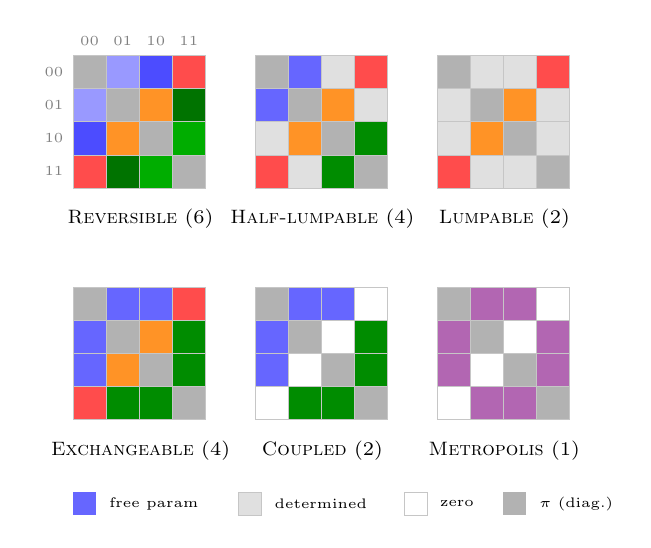
\begin{tikzpicture}[x=0.42cm,y=0.42cm,font=\scriptsize,
   cell/.style={draw=gray!45,line width=0.2pt}]
% row-major cells per panel: 00[pi,e1,e2,e5] 01[e1,pi,e6,e3] 10[e2,e6,pi,e4] 11[e5,e3,e4,pi]
\newcommand{\pnl}[4]{\begin{scope}[shift={(#1,#2)}]
  \foreach \col [count=\ii from 0] in {#4}{
     \pgfmathtruncatemacro{\rr}{3-int(\ii/4)}\pgfmathtruncatemacro{\cc}{mod(\ii,4)}
     \fill[\col] (\cc,\rr) rectangle ++(1,1);\draw[cell] (\cc,\rr) rectangle ++(1,1);}
  \node[anchor=north,align=center,text width=2.6cm] at (2,-0.35){#3};
\end{scope}}
% top row: Reversible, Half-lumpable, Lumpable
\pnl{0}{7}{\Reversible\ (6)}{black!30,blue!40,blue!70,red!70, blue!40,black!30,orange!85,green!45!black, blue!70,orange!85,black!30,green!68!black, red!70,green!45!black,green!68!black,black!30}
\pnl{5.5}{7}{\Halflump\ (4)}{black!30,blue!60,black!12,red!70, blue!60,black!30,orange!85,black!12, black!12,orange!85,black!30,green!55!black, red!70,black!12,green!55!black,black!30}
\pnl{11}{7}{\Lumpm\ (2)}{black!30,black!12,black!12,red!70, black!12,black!30,orange!85,black!12, black!12,orange!85,black!30,black!12, red!70,black!12,black!12,black!30}
% bottom row: Exchangeable, Coupled, Metropolis
\pnl{0}{0}{\Exchm\ (4)}{black!30,blue!60,blue!60,red!70, blue!60,black!30,orange!85,green!55!black, blue!60,orange!85,black!30,green!55!black, red!70,green!55!black,green!55!black,black!30}
\pnl{5.5}{0}{\Coupledm\ (2)}{black!30,blue!60,blue!60,white, blue!60,black!30,white,green!55!black, blue!60,white,black!30,green!55!black, white,green!55!black,green!55!black,black!30}
\pnl{11}{0}{\Metrop\ (1)}{black!30,violet!60,violet!60,white, violet!60,black!30,white,violet!60, violet!60,white,black!30,violet!60, white,violet!60,violet!60,black!30}
% state labels, on the top-left panel only
\foreach \s [count=\k from 0] in {11,10,01,00}{\node[left,gray] at (0,\k+0.5+7){\tiny\s};}
\foreach \s [count=\k from 0] in {00,01,10,11}{\node[above,gray] at (\k+0.5,4+7){\tiny\s};}
% legend, one row under the panels
\begin{scope}[shift={(0,-2.9)}]
  \fill[blue!60](0,0)rectangle++(0.7,0.7);\node[right]at(0.8,0.35){\tiny free param};
  \fill[black!12](5,0)rectangle++(0.7,0.7);\draw[cell](5,0)rectangle++(0.7,0.7);\node[right]at(5.8,0.35){\tiny determined};
  \fill[white](10,0)rectangle++(0.7,0.7);\draw[cell](10,0)rectangle++(0.7,0.7);\node[right]at(10.8,0.35){\tiny zero};
  \fill[black!30](13,0)rectangle++(0.7,0.7);\node[right]at(13.8,0.35){\tiny $\pi$ (diag.)};
\end{scope}
\end{tikzpicture}}
\end{minipage}\hfill
\begin{minipage}[c]{0.37\textwidth}
\caption{\textbf{The pair parameterizations, on the binary two-site chain.} Each
$4\times4$ block is the flux tensor over states $00,01,10,11$: diagonal is the stationary
$\pi$, off-diagonal the six symmetric edge fluxes---four single-site flips and two
simultaneous flips (correlated $00\!\leftrightarrow\!11$, swap
$01\!\leftrightarrow\!10$). Color marks each free flux parameter (count in
parentheses); reversibility holds throughout. Component
exchangeability ties the two single-flip pairs (\Exchm); the
\CTBN/\Coupledm\ restriction zeroes the double flips; \Metrop\ collapses all single flips
to one shared exchangeability; two-sided \Lumpm\ frees the two double flips and
\emph{determines} the singles from $\pi$ and \Cref{eq:lump}; one-sided \Halflump\ drops
the swap tie and constrains one coordinate only. \Coupledm\ and \Lumpm\ both keep two
free parameters, but on complementary edges.
}
\label{fig:params}

{\footnotesize\itshape Alt text: Six square grids in two rows of three, one per parameterization, each a four-by-four block over the states 00, 01, 10 and 11. Cells are colored to show which flux parameters are free, which are determined by the stationary distribution, which are zero, and which are the stationary diagonal.}
\end{minipage}
\end{figure}
We now generalize from two binary components to full length sequences.
Let two coupled sites evolve as a \CTMC\ on ordered pairs
$\Xset^2$, with states $x=(i,j)$, $y=(k,l)$.
Write the stationary distribution $\pi_{ij}>0$ and the off-diagonal stationary
fluxes $F_{xy}=\pi_xQ_{xy}$.
The pair chain is the chain of \Cref{sec:single} on a larger state space:
$\pi$ is over $A^2$ states, and
$Q$ describes $A^2\times A^2$ possible transitions.

\paragraph{The Klein group on the flux tensor.} Component exchangeability
restricts $\pi_{ij}=\pi_{ji}$; reversibility and exchangeability of the fluxes
enforce $F_{ij,kl}=F_{kl,ij}$ and $F_{ij,kl}=F_{ji,lk}$, respectively. Let
$\mathsf{R}(i,j;k,l)=(k,l;i,j)$ reverse the transition, $\mathsf{E}(i,j;k,l)=(j,i;l,k)$
swap the two components, and $\mathsf{RE}(i,j;k,l) = (l,k;j,i)$ be a composition of the two operations. The Klein four-group $G=\{\mathsf{e}, \mathsf{R}, \mathsf{E}, \mathsf{RE} \}\cong V_4$
acts on directed off-diagonal transitions.
Assigning one nonnegative variable $\phi_o$ per orbit $o$ makes every reversibility and
exchangeability equality automatic. Burnside's lemma counts the orbits as
$|\mathcal O|=(A^4+A^2-2A)/4$.

\paragraph{Lumpability versus single-component transitions.} We now consider two
different specializations of the pair chain.
(1) A continuous-time Bayes network
(\CTBN)~\citep{nodelman2002,cohn2010} forbids simultaneous transitions at
the two sites: every jump changes one component, so a compensatory
double-substitution must pass through a transiently unfavorable
intermediate. (2) A lumpable model, by contrast, is one which can be projected
to a single component without losing the Markov property, implying
\begin{equation}
\label{eq:lump}
\sum_l F_{ij,kl}=\frac{\pi_{ij}}{\rho_i}\,g_{ik},\qquad i\ne k,
\qquad \rho_i=\sum_j\pi_{ij},
\end{equation}
with $g_{ik}=g_{ki}\ge0$ the symmetric marginal edge fluxes and
$\Theta_{ik}=g_{ik}/\rho_i$ the marginal generator; exchangeability then gives
lumpability of the second coordinate for free. Written compactly,
\Cref{eq:lump} is $N\phi=\Xi(\pi)g$, with $N$ the sparse incidence map
summing orbit fluxes $\phi$ over $l$ and $\Xi(\pi)$ the diagonal ratio map
$\pi_{ij}/\rho_i$. The two are generically incompatible: \revised{chains restricted to} single-component
transitions cannot \deleted{also} be lumpable under projection to either component \revised{unless $\pi$ factorizes}.
Biologically the \CTBN\ excludes compensatory double-substitutions---the
tension familiar from codon models, where the data favor simultaneous
change~\citep{KosiolHolmesGoldman2007}.

\paragraph{Coupled amino acid models used in this study.}  \Exchm\ is the reversible,
exchangeable, 400-state general chain over all Klein orbits. This model has as many free
flux parameters as it does orbits, $(A^4+A^2-2A)/4$.
We evaluate two types of \CTBN s: \Coupledm\ and \Metrop. The \Coupledm\
model is simply the single-transition chain through Klein orbits; it has $A^2(A-1) / 2$
free flux parameters.
The \Metrop\ family uses the generator
$Q_{ij,kj}=S_{ik}\,f(\pi_{ij},\pi_{kj})$ and $Q_{ij,il}=S_{jl}\,f(\pi_{ij},\pi_{il})$, with
symmetric $A\times A$ exchangeability matrix $S$ and reversible rate kernel $f(\pi_x,\pi_y)$.
All \Metrop\ models have $A(A-1) / 2$ free flux parameters (i.e. exchangeabilities in $S$).
We consider four reversible kernels
$f$:  the square root $\sqrt{\pi_y/\pi_x}$, the GTR $\pi_y$, Barker $\pi_y/(\pi_x{+}\pi_y)$, and
Hastings $\min(1,\pi_y/\pi_x)$.

We also fit the two lumpable chains of \Cref{eq:lump}. \Lumpm\ is \Exchm\ constrained
to two-sided lumpability, leaving $32{,}870$ free flux parameters; \Halflump\ drops the
exchangeability tie and is lumpable on the first component only, leaving $72{,}390$.

For all paired models except \Halflump, the symmetric stationary distribution has
$A(A{+}1)/2-1$ free probabilities. \Halflump, not being exchangeable, has the full
$A^2-1$.

\paragraph{The shared E-step and model-specific M-step.} All paired models share the
same E-step, which computes transition usages $U_{xy}$ and dwell times $T_x$
from the bridge statistics in \eqref{eq:bridge}.
Derived ancestral counts are $V'_x=V_x+\sum_{y\ne x}U_{yx}$, as used in \eqref{eq:ell2}.
The expected complete-data log-likelihood is $\ell(Q, \pi) = \sum_x
V'_x\log\pi_x + \sum_{x\ne y}U_{xy}\log Q_{xy}-\sum_xT_x\!\sum_{y \neq x}Q_{xy}$.

We generally implement the M-step by expectation-conditional maximization, alternating a
closed-form update for flux parameters at fixed $\pi$ with a numerical $\pi$-update at fixed
flux values until convergence.
For the \Exchm\ model M-step, assign one flux parameter $\phi_o$ to each Klein-group orbit $o$.
At fixed $\pi$, the orbit flux has closed-form update
$\widehat\phi_o=C_o/H_o(\pi), C_o=\sum_{(x,y)\in o}U_{xy}$, $H_o(\pi)=\sum_{(x,y)\in o} T_x/\pi_x$.
The \Coupledm\ M-step uses the same orbit-flux update but is restricted to
single-component transitions.
The \Metrop\ M-step pools over the unchanging residue $j$ and over both sites,
since $S$ depends on neither. At fixed $\pi$ for residues $m,n \in \Xset$, let
$C_{mn}=\sum_j\big(U_{mj,nj}+U_{jm,jn}\big)$
and $H_{mn}(\pi)=\sum_j\big(T_{mj}f(\pi_{mj},\pi_{nj})+T_{jm}f(\pi_{jm},\pi_{jn})\big)$.
Then, the $S$-block update follows a similar ratio form as the previous models:
$\widehat S_{mn}=(C_{mn}{+}C_{nm})/[H_{mn}(\pi){+}H_{nm}(\pi)]$.

Lumpability is the hard case: its constraint $N\phi=\Xi(\pi)g$~\eqref{eq:lump} ties flux
and stationary bilinearly, turning even the flux block into a constrained solve with
multipliers $\lambda$ (the rational Sinkhorn update
$\phi_o=C_o/[H_o(\pi)+(N^\top\lambda)_o]$, rational not exponential because the \CTMC\
complete data is Poisson), and leaves $\pi$ without closed form, so it needs a
bilinear/ECM alternation of the constrained flux and $\pi$ steps.

% =============================================================
\subsection{Many components and variational inference}
\label{sec:multi}
% =============================================================

The pair models have $A^2$ states, but this grows to $A^L$ for a cluster of $L$ coupled sites. Exact
matrix exponentiation does not simplify for the general \CTBN.
Existing phylogenetic approaches to this scaling problem use context-dependent chains,
ML/MCMC-EM estimators, and variational or truncation
 bounds~\citep{ArndtBurgeHwa2003NeighborDependent,ChristensenHobolthJensen2005PseudoLikelihood,Hobolth2008MCMCEM,JensenPedersen2000ContextDependent,JojicEtAl2004PhyloHMM,LunterHein2004NearestNeighbor,MathewsSchmidler2025ImportanceSampling,MatsenRalph2022BoundingDependency,SiepelHaussler2004ContextML,WexlerGeiger2007VariationalUpper}.
We take the variational law to be a product of independent single-site \CTMC\
bridges~\citep{cohn2010}. The bound is written in the sufficient statistics~\eqref{eq:bridge} of
the $A^L$ product chain, but these collapse to a boundary term and a one-dimensional
integral over single-site bridge marginals: polynomial, not exponential, in cluster size.

\paragraph{Path ELBO.} Let a cluster of $L$ sites carry the Potts target
$\Pi(x)\propto e^{-E(x)}$, $x\in\Xset^L$, with
$E(x)=-\sum_s h_s(x_s)-\sum_{s<s'}H_{ss'}(x_s,x_{s'})$, and let the independent
single-site GTR proposal $R_{ic}=S_{ic}\pi_c$ act site-wise (i.e. $R$ is $A \times A$, and $\pi$ is over $A$ states).
Suppose the target rate for the move $x\to x^{s:c}$ (i.e. replacing residue $i=x_s$ at site $s$ with $c$) takes the square-
root\footnote{
Among acceptances $A(z)\propto z^\theta$, reversibility ($A(z)=zA(1/z)$) forces
$\theta=\tfrac12$: the square root is the unique log-linear reversible acceptance, i.e.\
the only one for which $\log(W/B)$ is a potential difference~\eqref{eq:logWB}.
}
\Metrop\ form
\begin{equation}\label{eq:sqrtmet}
 W_{x,x^{s:c}}=R_{ic}\sqrt{\tfrac{\Pi(x^{s:c})R_{ci}}{\Pi(x)R_{ic}}}
 =S_{ic}\sqrt{\pi_i\pi_c}\;e^{-\frac12\Delta^c_sE(x)},\qquad
 \Delta^c_sE(x)=E(x^{s:c})-E(x),
\end{equation}
reversible w.r.t.\ $\Pi$ for any $S,h,H$.  $W$ has size $A^L \times A^L$.

The branch likelihood would require \revised{the} matrix exponential $(e^{tW})_{ab}$, but $W$ does not factorize across sites and \revised{its exponential} costs $A^{3L}$ to compute.
However, the likelihood can be bounded from below by assuming each site evolves independently.
Accordingly, let $B$ be our variational
proposal\footnote{
As described here, the proposal is fixed; it can be made variational, e.g. by introducing midpoint-node distributions.
}
that uses the product of independent $R$-chains, with size $A^L \times A^L$.

On a branch of length $t$ with $x(0)=a$, $x(t)=b$,
Girsanov's formula for jump processes writes the log-density ratio of the two path
measures as a difference of \emph{complete-data} log-likelihoods of the
form~\eqref{eq:cdl}.
A trajectory $\mathbb X$ with usages $U$ and dwell times $T$ has
\begin{equation}\label{eq:girsanov}
 \log\frac{d P_W}{d P_B}(\mathbb X)=\ell_W(\mathbb X)-\ell_B(\mathbb X),
 \qquad
 \ell_Q(\mathbb X)=\sum_{x\ne y}U_{xy}\log Q_{xy}-\sum_xT_x\,q(x),
\end{equation}
with $q(x)=\sum_{y\ne x}Q_{xy}$ the exit rate. The ELBO adds the $B$-bridge average of this
difference to the proposal's own log-transition probability,
\begin{equation}\label{eq:pathelbo}
 \mathcal L_{ab}=\sum_s\log[e^{tR}]_{a_sb_s}
 +\sum_{x,s,c\ne x_s}\bar U^{ab}_{x,s:c}\log\frac{W_{x,x^{s:c}}}{B_{x,x^{s:c}}}
 -\sum_x\bar T^{ab}_x\,[w(x)-\beta(x)],
\end{equation}
where $w(x)=\sum_{s,c}W_{x,x^{s:c}}$ and $\beta(x)=\sum_{s,c}B_{x,x^{s:c}}$ are the two exit rates
and $\bar T,\bar U$ are the expected dwell and usage bridge statistics~\eqref{eq:bridge} of the
$A^L$-state product chain. Jensen's inequality gives
$\mathcal L_{ab}\le\log[e^{tW}]_{ab}$.

Equation~\eqref{eq:pathelbo} is the mean-field free energy of Cohn et
al.~\citep{cohn2010} at one member of their factored family, and is consistent with their Theorem~3:
where Cohn et al. optimize a time-varying \emph{inhomogeneous} rate via Euler--Lagrange ODEs, we consider the product of single-site
bridges of the \emph{time-homogeneous} $R$. Fixing the rates, rather than
solving their ODEs, makes ours the looser of the two bounds, but more stable to compute: the terms that diverge as $u\to t$
(their rate integral divides by a backward probability vanishing at the endpoint)
telescope analytically into the $\sum_s\log[e^{tR}]_{a_sb_s}$ normalizer, leaving a smooth
integrand. The partition function of
$\Pi$ cancels from every rate ratio in \eqref{eq:sqrtmet}, entering only the root factor
of the tree likelihood. Both contractions below rely on log-linearity making the log-rate
ratio a \emph{potential difference},
\begin{equation}\label{eq:logWB}
 \log\frac{W_{x,x^{s:c}}}{B_{x,x^{s:c}}}=\psi(x^{s:c})-\psi(x),
 \qquad
 \psi(x)=-\tfrac12\sum_s\log\pi_{x_s}-\tfrac12E(x).
\end{equation}


\paragraph{Contraction to single-site bridge marginals.} The statistics $\bar T,\bar U$ are
joint over $A^L$ and do \emph{not} factorize, but both terms of \eqref{eq:pathelbo}
reduce to per-site quantities, for two different consequences of~\eqref{eq:logWB}.

\emph{The usage term is a boundary term.} Every jump of the product chain moves one site,
so along any path $a=x_0\to\cdots\to x_K=b$ the increments $\psi(x_k)-\psi(x_{k-1})$
telescope to $\psi(b)-\psi(a)$: the same value for every path, whatever its length or
order. Since $\sum_{x,s,c}\bar U^{ab}_{x,s:c}f$ (for generic function $f$)\revised{~}is by definition the bridge
expectation of $\sum_{\mathrm{jumps}}f$, and the expectation of a path-independent
quantity is that quantity,
\begin{equation}\label{eq:telescope}
 \sum_{x,\,s,\,c\ne x_s}\bar U^{ab}_{x,s:c}\log\frac{W_{x,x^{s:c}}}{B_{x,x^{s:c}}}
 =\tfrac12\sum_s\log\frac{\pi_{a_s}}{\pi_{b_s}}+\tfrac12\big[E(a)-E(b)\big].
\end{equation}

\emph{The dwell term contracts to a one-dimensional integral.} The product chain has
$M_{ab}(t)=\prod_sM^s_{a_sb_s}(t)$, so \eqref{eq:bridge} gives
$\bar T^{ab}_x=\int_0^t\prod_sp^s_u(x_s)\,du$ and hence, for any $\phi$,
\begin{equation}\label{eq:contract}
 \sum_x\bar T^{ab}_x\,\phi(x)=\int_0^t\!\E_u[\phi]\;du,
 \qquad
 p^s_u(y)=\frac{M^s_{a_sy}(u)\,M^s_{yb_s}(t-u)}{M^s_{a_sb_s}(t)},
\end{equation}
with $M^s(u)=e^{uR}$ and $\E_u$ the expectation under the product measure
$\prod_sp^s_u$: the joint sum has become a time integral of an expectation over
\emph{independent} sites. Now $-\tfrac12\Delta^c_sE(x)$ is a sum over the neighbors of
$s$, so \revised{$W_{x,x^{s:c}}$} is a \emph{product} over them, and the expectation of a product of functions
of distinct independent sites is the product of the expectations,
\begin{equation}\label{eq:sep}
 \E_u\big[W_{x,x^{s:c}}\big]=\sum_i p^s_u(i)\,S_{ic}\sqrt{\pi_i\pi_c}\;
   e^{\frac12[h_s(c)-h_s(i)]}
   \prod_{s'\ne s}\Big(\sum_z p^{s'}_u(z)\;e^{\frac12[H_{ss'}(c,z)-H_{ss'}(i,z)]}\Big).
\end{equation}
Every factor is a single sum over one site's alphabet, so the $A^L$ configuration sum
never forms, even though the exit rate depends on all neighbors jointly and nonlinearly:
separability across neighbors, not linearity, is what is required. The proposal exit rate
$\beta$ is one-body and contracts likewise.
At each quadrature node, evaluating \eqref{eq:sep} costs $O(A^3)$ per contact and $O(A^2)$
per site, so the ELBO costs $O\!\big(m(LA^2+|\mathcal C|A^3)\big)$ for $m$ quadrature nodes
and $|\mathcal C|$ contacts (the coupled pairs $s<s'$ with $H_{ss'}\ne0$): polynomial in
cluster size rather than exponential.

\paragraph{When the time integral is exact.} Factorization across sites is not
factorization across time, so \eqref{eq:contract} leaves a genuine integral. Each
$p^s_u$ is a sum of $A^2$ exponentials in $u$, so the integrand of \eqref{eq:sep} is a
product of one such sum per coupled site, $L$ in all. For $L=2$ the integral is the
divided-difference kernel~\eqref{eq:bridgestat} and $\mathcal L_{ab}$ is
exactly closed-form---the regime of \Cref{fig:elbovsexpm}. Larger clusters give $A^{2L}$
terms and we integrate numerically instead. Its exponents are those of $R$, so it is
entire and Gauss--Legendre converges spectrally: with $R$ set to LG08, $m\le14$ nodes reach
machine precision for $L\le5$, $t\le3$ and couplings up to $|H|\sim4$. This conditioning separates
the bound from the inhomogeneous mean field, whose endpoint-singular integrand converges
at first order.


%% The notation subsection below was an appendix in earlier versions of this
%% paper.  Molecular Biology and Evolution sets no page limit, so it is folded
%% into Materials and Methods rather than shipped as supplementary material.
%% Its text is unchanged.


%% Shared column layout for every notation table below.

\subsection{Notation}
\label{app:notation}

\Cref{tab:not-single,tab:not-binary,tab:not-pair,tab:not-compare,tab:not-multi}
list every symbol introduced in \Cref{sec:single,sec:pair,sec:paircompare,sec:multi}. Throughout, $A=|\Xset|$ is the alphabet size ($A=20$ for amino
acids), $t$ is a branch length, and $u$ is time within a branch, $0\le u\le t$. The
size column is filled in only for vectors, matrices, tensors and index sets; a dash
marks a scalar, an operator, or an object with no fixed dimension. Where a section
reuses a symbol from an earlier section at a new size, the row is repeated at that
size.

% -------------------------------------------------------------
\begingroup
\setlength{\tabcolsep}{4pt}
\renewcommand{\arraystretch}{1.15}
\begin{longtable}{@{}YZX@{}}
\caption{Notation of \Cref{sec:single} (single-site models).}
\label{tab:not-single}\\
\notationhead
\endfirsthead
\multicolumn{3}{@{}l}{\itshape \Cref{tab:not-single}, continued.}\\
\notationhead
\endhead
\bottomrule
\endlastfoot
$\Xset$ & $A$ & The sequence alphabet; $A=|\Xset|=20$ for amino acids\\
$x,y$ & \nodim & States of the single site, $x,y\in\Xset$; $x$ the source and $y$ the destination of a transition\\
$a,b$ & \nodim & Endpoint states of a branch: $X(0)=a$ at the ancestor, $X(t)=b$ at the descendant\\
$t$ & \nodim & Branch length\\
$u$ & \nodim & Time within a branch, $0\le u\le t$\\
$Q$ & $A\times A$ & Generator of the single-site \CTMC, with $Q_{xy}\ge0$ off-diagonal and $Q_{xx}=-\sum_{y\ne x}Q_{xy}$\\
$\pi$ & $A$ & Equilibrium distribution; reversibility is $\pi_xQ_{xy}=\pi_yQ_{yx}$\\
$\widetilde Q$ & $A\times A$ & Symmetrized generator $\widetilde Q_{xy}=Q_{xy}\sqrt{\pi_x/\pi_y}$, real and symmetric\\
$\xi_k$ & \nodim & The $k$-th eigenvalue of $\widetilde Q$, with $\xi_k\le0$\\
$v^{(k)}$ & $A$ & The $k$-th eigenvector of $\widetilde Q$, from $\widetilde Q=\sum_k\xi_kv^{(k)}{v^{(k)}}^\top$\\
$P(y\mid x,t)$ & \nodim & Probability of ending at $y$ after time $t$ from $x$, \eqref{eq:pt}\\
$M(t)$ & $A\times A$ & The matrix exponential $e^{Qt}$, so $P(y\mid x,t)=M_{xy}(t)$\\
$M_{ab}(t)$ & \nodim & Endpoint likelihood of the branch: the normalizer of the bridge expectations \eqref{eq:bridge}\\
$S$ & $A\times A$ & GTR exchangeabilities, $S=S^\top$, with $Q_{xy}=S_{xy}\pi_y$; LG08 is one such $S$\\
$\mathbb X$ & \nodim & A branch trajectory $(X(u))_{0\le u\le t}$: the complete data for one branch\\
$T_x$ & $A$ & Dwell time in state $x$ along a trajectory (a sufficient statistic)\\
$U_{xy}$ & $A\times A$ & Usage count of the transition $x\to y$ along a trajectory (a sufficient statistic)\\
$\ell(Q)$ & \nodim & Complete-data log-likelihood of a trajectory given $X(0)$ and $Q$, \eqref{eq:cdl}\\
$\E[\,\cdot\mid a,b\,]$ & \nodim & Expectation over trajectories conditioned on the two branch endpoints\\
$\bar T^{ab}_x$ & $A$ & Endpoint-conditioned expected dwell time, \eqref{eq:bridge}\\
$\bar U^{ab}_{xy}$ & $A\times A$ & Endpoint-conditioned expected transition usage, \eqref{eq:bridge}\\
$I^{ab}_{xy}(t)$ & $A\times A$ & Time convolution $\int_0^tM_{ax}(u)M_{yb}(t{-}u)\,du$: the unnormalized bridge statistic\\
$D^{kl}(t)$ & $A\times A$ & Exponential divided-difference kernel \eqref{eq:bridgestat}, indexed by the eigenvalues of $\widetilde Q$; evaluates $I^{ab}_{xy}(t)$ in the spectral basis\\
$V_x$ & $A$ & Count of the ancestral state, the event $X(0)=x$\\
$V'_x$ & $A$ & Derived ancestral count $V_x+\sum_{y\ne x}U_{yx}$: every entry into $x$, root included\\
$\ell(S,\pi)$ & \nodim & Complete-data log-likelihood including the root, \eqref{eq:ell2}\\
$\widehat S_{xy}$ & $A\times A$ & Closed-form M-step maximizer of $S$ at fixed $\pi$, $(U_{xy}{+}U_{yx})/(T_x\pi_y+T_y\pi_x)$\\
$\sigma_y$ & $A$ & Total exchangeability out of $y$, $\sigma_y=\sum_{z\ne y}S_{yz}$\\
$V''_x$ & $A$ & Expected number of latent $\pi$-tokens equal to $x$ drawn for rejected moves under the secret-destination augmentation\\
$\widehat\pi_x$ & $A$ & Fixed-point M-step update of $\pi$, $\widehat\pi_x\propto V'_x+V''_x$\\
\end{longtable}
\endgroup

% -------------------------------------------------------------
\begingroup
\setlength{\tabcolsep}{4pt}
\renewcommand{\arraystretch}{1.15}
\begin{longtable}{@{}YZX@{}}
\caption{Notation of \Cref{sec:pairbinary} (the pair of telegraph processes). For the
four model rows the size column gives the number of free flux parameters.}
\label{tab:not-binary}\\
\notationhead
\endfirsthead
\notationhead
\endhead
\bottomrule
\endlastfoot
$i,j$ & \nodim & The two binary components, $i,j\in\{0,1\}$\\
$00,01,10,11$ & $4$ & State space of the coupled telegraph pair\\
\Reversible & $6$ & The reversible binary pair chain: twelve flux parameters reduced to six by reversibility\\
\Exchm & $4$ & \Reversible\ with the flux exchangeability constraint added\\
\Coupledm & $2$ & The asynchronous (\CTBN) specialization: simultaneous flips forbidden\\
\Metrop & $1$ & \Coupledm\ with the proposal fixed, leaving one rate to set the time scale\\
\Halflump & $4$ & Lumpable on the first component only: the swap tie is dropped and one coordinate constrained\\
\Lumpm & $2$ & Exchangeably lumpable, projectable onto either component: the two simultaneous flips are free and the four single flips determined by $\pi$, \eqref{eq:lump}\\
$\pi_{01}=\pi_{10}$ & \nodim & The stationary exchangeability constraint; together with normalization it leaves two free stationary parameters, the mean and the covariance\\
\end{longtable}
\endgroup

% -------------------------------------------------------------
\begingroup
\setlength{\tabcolsep}{4pt}
\renewcommand{\arraystretch}{1.15}
\begin{longtable}{@{}YZX@{}}
\caption{Notation of \Cref{sec:pairgeneral} (the general pair chain). For the three
model rows the size column gives the number of free flux parameters.}
\label{tab:not-pair}\\
\notationhead
\endfirsthead
\multicolumn{3}{@{}l}{\itshape \Cref{tab:not-pair}, continued.}\\
\notationhead
\endhead
\bottomrule
\endlastfoot
$\Xset^2$ & $A^2$ & State space of the pair chain: ordered residue pairs, $A^2=400$\\
$x=(i,j)$, $y=(k,l)$ & \nodim & Pair states; $i,j,k,l\in\Xset$ are the residues at the two sites\\
$\pi_{ij}$ & $A\times A$ & Stationary distribution over pair states, $\pi_{ij}>0$; exchangeability forces $\pi_{ij}=\pi_{ji}$, leaving $A(A{+}1)/2-1=209$ free probabilities\\
$Q$ & $A^2\times A^2$ & Generator of the pair chain\\
$F_{xy}$ & $A^2\times A^2$ & Off-diagonal stationary flux $F_{xy}=\pi_xQ_{xy}$; reversibility is $F_{ij,kl}=F_{kl,ij}$ and flux exchangeability is $F_{ij,kl}=F_{ji,lk}$\\
$\mathsf R$ & \nodim & Reversal of a directed transition, $\mathsf R(i,j;k,l)=(k,l;i,j)$\\
$\mathsf E$ & \nodim & Component swap, $\mathsf E(i,j;k,l)=(j,i;l,k)$\\
$\mathsf{RE}$ & \nodim & Composition of the two, $\mathsf{RE}(i,j;k,l)=(l,k;j,i)$\\
$G$ & $4$ elements & The Klein four-group $\{\mathsf e,\mathsf R,\mathsf E,\mathsf{RE}\}\cong V_4$, acting on directed off-diagonal transitions\\
$o$ & \nodim & One orbit of $G$ on the directed off-diagonal transitions\\
$\mathcal O$ & $(A^4{+}A^2{-}2A)/4$ & The set of Klein orbits, counted by Burnside's lemma; $40{,}090$ at $A=20$\\
$\phi_o$ & $|\mathcal O|$ & The nonnegative flux assigned to orbit $o$; one per orbit makes every reversibility and exchangeability equality automatic\\
$S$ & $A\times A$ & Symmetric exchangeabilities of the \Metrop\ family, shared by both sites and independent of the unchanging residue\\
$f(\pi_x,\pi_y)$ & \nodim & Reversible rate kernel of the \Metrop\ family: square root $\sqrt{\pi_y/\pi_x}$, GTR $\pi_y$, Barker $\pi_y/(\pi_x{+}\pi_y)$, or Hastings $\min(1,\pi_y/\pi_x)$\\
\Exchm & $(A^4{+}A^2{-}2A)/4$ & The reversible, exchangeable general chain on residue pairs: one flux parameter per Klein orbit\\
\Coupledm & $A^2(A{-}1)/2$ & The \CTBN\ restriction of \Exchm: single-component transitions only, every simultaneous-transition flux zero\\
\Metrop & $A(A{-}1)/2$ & The kernel family $Q_{ij,kj}=S_{ik}f(\pi_{ij},\pi_{kj})$ and $Q_{ij,il}=S_{jl}f(\pi_{ij},\pi_{il})$\\
\Lumpm & $32{,}870$ & \Exchm\ constrained to two-sided lumpability, \eqref{eq:lump}\\
\Halflump & $72{,}390$ & The reversible, non-exchangeable chain constrained to lumpability on the first component only; its stationary is the full $A^2{-}1$, not the symmetric $A(A{+}1)/2-1$\\
$\rho_i$ & $A$ & Marginal stationary of the first component, $\sum_j\pi_{ij}$, \eqref{eq:lump}\\
$g_{ik}$ & $A\times A$ & Symmetric marginal edge fluxes of the lumped chain, $g_{ik}=g_{ki}\ge0$\\
$\Theta_{ik}$ & $A\times A$ & Marginal generator of the lumped chain, $g_{ik}/\rho_i$\\
$N$ & \nodim & Sparse incidence map summing orbit fluxes over the second component; \eqref{eq:lump} reads $N\phi=\Xi(\pi)g$\\
$\Xi(\pi)$ & \nodim & Diagonal ratio map $\pi_{ij}/\rho_i$ in that compact form\\
$\lambda$ & \nodim & Multipliers of the lumpability constraint in the \Lumpm\ M-step\\
$T_x$ & $A^2$ & Pair-state dwell times, from the bridge statistics \eqref{eq:bridge}\\
$U_{xy}$ & $A^2\times A^2$ & Pair-state transition usages, from the same bridge statistics\\
$V_x$, $V'_x$ & $A^2$ & Ancestral pair-state count and its derived form $V'_x=V_x+\sum_{y\ne x}U_{yx}$\\
$\ell(Q,\pi)$ & \nodim & Expected complete-data log-likelihood of the pair chain, shared by all pair models\\
$C_o$ & $|\mathcal O|$ & Orbit-summed usage $\sum_{(x,y)\in o}U_{xy}$: the numerator of the orbit-flux M-step\\
$H_o(\pi)$ & $|\mathcal O|$ & Orbit-summed dwell weight $\sum_{(x,y)\in o}T_x/\pi_x$: the denominator of the orbit-flux M-step\\
$\widehat\phi_o$ & $|\mathcal O|$ & Closed-form orbit-flux update $\widehat\phi_o=C_o/H_o(\pi)$ at fixed $\pi$\\
$m,n$ & \nodim & Residues $m,n\in\Xset$ indexing the \Metrop\ M-step\\
$C_{mn}$ & $A\times A$ & $\sum_j(U_{mj,nj}+U_{jm,jn})$: usage pooled over the unchanging residue $j$ and over both sites\\
$H_{mn}(\pi)$ & $A\times A$ & $\sum_j\big(T_{mj}f(\pi_{mj},\pi_{nj})+T_{jm}f(\pi_{jm},\pi_{jn})\big)$: the matching pooled dwell weight\\
$\widehat S_{mn}$ & $A\times A$ & Closed-form \Metrop\ M-step update $(C_{mn}{+}C_{nm})/[H_{mn}(\pi){+}H_{nm}(\pi)]$\\
\end{longtable}
\endgroup

% -------------------------------------------------------------
\begingroup
\setlength{\tabcolsep}{4pt}
\renewcommand{\arraystretch}{1.15}
\begin{longtable}{@{}YZX@{}}
\caption{Notation of \Cref{sec:paircompare} (comparing the pair couplings), covering
the fitted models, the count corpus, and the two result tables.}
\label{tab:not-compare}\\
\notationhead
\endfirsthead
\multicolumn{3}{@{}l}{\itshape \Cref{tab:not-compare}, continued.}\\
\notationhead
\endhead
\bottomrule
\endlastfoot
$K$ & \nodim & Number of components in a \Metrop\ mixture; $K=4$ and $K=8$ are fitted\\
transposed & \nodim & A non-exchangeable mixture in which each component is entered twice, once as itself and once transposed, with the two orientations tied to one parameter set and weighted equally\\
$\Gamma+I$ & $4{+}1$ & The rate model used by every fitted model: four discrete $\Gamma$ categories plus an invariant class, with a shared branch-length multiplier per family\\
LG08$\otimes$LG08 & \nodim & Null model: the independent product of two LG08 chains, which keeps the dynamics and discards the coupling\\
$n(i,j;k,l;t)$ & $A^2\times A^2$ per bin & The coupled substitution count tensor; $t$ is a binned branch-length coordinate set by maximum-likelihood pairwise distance under LG08\\
C$\beta$, separation & \nodim & The contact definition: C$\beta$ distance below $8$ \AA\ and at least $7$ residues apart in the primary sequence\\
train LL, val LL & \nodim & Mean per-transition log-likelihood in nats on the $80\%$ training and $20\%$ held-out splits\\
$\mathrm{MI_{stat}}$ & \nodim & Mutual information between the two sites under the fitted stationary $\pi$, in nats\\
$\mathrm{MI_{dyn}}$ & \nodim & Mutual information of the ancestor--descendant joint $\pi_xM_{xy}(t)$, in nats\\
Flux, Prob. & \nodim & The two free-parameter counts of \Cref{tab:pairfit}: rates and exchangeabilities, and the stationary $\pi$ together with any mixture weights\\
Q2 & $79{,}800+399$ & CherryML's fitted $400$-state coupled matrix, used as an external baseline; reversible, hence half the $\sim\!160{,}000$ entries of a general $400$-state generator\\
$c$ & \nodim & Index of a fitted mixture component, i.e.\ one interaction class\\
$w$ & $K$ & Mixture weight of class $c$; the panels of \Cref{fig:components} are sorted by it\\
$\pi_c(a,b)$ & $A\times A$ & Stationary distribution of class $c$ over residue pairs $(a,b)$, with $a,b\in\Xset$\\
$\rho_a$ & $A$ & Marginal of $\pi_c$ at one site; the coupling plotted in \Cref{fig:components} is $\log[\pi_c(a,b)/\rho_a\rho_b]$\\
$\mathrm{MI}(\pi_c)$ & \nodim & Stationary mutual information of a single class\\
$v(a)$ & $A$ & Biophysical property score of residue $a$ on one of four axes (charge, Kyte--Doolittle hydropathy, volume, aromaticity), standardized to the pooled amino-acid frequencies\\
$\mathrm{Cov}_c$ & \nodim & Covariance of $v(a)$ and $v(b)$ under $\pi_c(a,b)$: the within-class coupling of class $c$ on one axis\\
Strength & \nodim & Mean of $|\mathrm{Cov}_c|$ over the classes, reported per axis in \Cref{tab:axes}\\
Within, Between, Pooled & \nodim & Decomposition of the pooled covariance into the mixture-weighted within-class term and the between-class term arising from compositional differences among classes\\
Per-class signs & $K$ & The sign of the within-class covariance in each of the $K{=}8$ classes: $\texttt{+}$, $\texttt{-}$, or $\texttt{0}$ for near zero\\
\end{longtable}
\endgroup

% -------------------------------------------------------------
\begingroup
\setlength{\tabcolsep}{4pt}
\renewcommand{\arraystretch}{1.15}
\begin{longtable}{@{}YZX@{}}
\caption{Notation of \Cref{sec:multi} (many components and variational inference).
Here $\pi$ and $S$ are single-site objects over $A$ states, not the pair-state objects
of \Cref{tab:not-pair}.}
\label{tab:not-multi}\\
\notationhead
\endfirsthead
\multicolumn{3}{@{}l}{\itshape \Cref{tab:not-multi}, continued.}\\
\notationhead
\endhead
\bottomrule
\endlastfoot
$L$ & \nodim & Number of sites in a coupled cluster; the joint chain has $A^L$ states\\
$s,s'$ & \nodim & Site indices within the cluster\\
$x$ & $A^L$ & A cluster configuration $x\in\Xset^L$, carrying residue $x_s$ at site $s$\\
$a,b$ & $A^L$ & Cluster configurations at the two branch endpoints, $x(0)=a$ and $x(t)=b$\\
$x^{s:c}$ & \nodim & The configuration $x$ with site $s$ changed from $i=x_s$ to $c$\\
$i,c$ & \nodim & The residue at site $s$ before and after a move, $i,c\in\Xset$\\
$z$ & \nodim & Summation index over the alphabet at a neighboring site $s'$\\
$\Pi(x)$ & $A^L$ & The Potts target $\Pi(x)\propto e^{-E(x)}$; its partition function cancels from every rate ratio and enters only the root factor of the tree likelihood\\
$E(x)$ & \nodim & Potts energy $-\sum_sh_s(x_s)-\sum_{s<s'}H_{ss'}(x_s,x_{s'})$\\
$h_s$ & $A$ & One-body field at site $s$\\
$H_{ss'}$ & $A\times A$ & Coupling between sites $s$ and $s'$\\
$\mathcal C$ & $|\mathcal C|$ & The set of contacts: the coupled pairs $s<s'$ with $H_{ss'}\ne0$\\
$\Delta^c_sE(x)$ & \nodim & Energy change of a single move, $E(x^{s:c})-E(x)$\\
$S$, $\pi$ & $A\times A$, $A$ & Exchangeabilities and equilibrium of the single-site proposal, over $A$ states\\
$R$ & $A\times A$ & The independent single-site GTR proposal generator $R_{ic}=S_{ic}\pi_c$, acting site-wise; set to LG08 in the numerical work\\
$W$ & $A^L\times A^L$ & The square-root \Metrop\ generator \eqref{eq:sqrtmet}, reversible with respect to $\Pi$ for any $S,h,H$; it does not factorize across sites\\
$A(z)$, $\theta$ & \nodim & The acceptance function $A(z)\propto z^\theta$ of the footnote to \eqref{eq:sqrtmet}; reversibility forces $\theta=\tfrac12$\\
$B$ & $A^L\times A^L$ & The variational proposal: the product of independent $R$-chains across the $L$ sites\\
$P_W$, $P_B$ & \nodim & The two path measures on a branch, whose log-density ratio is \eqref{eq:girsanov}\\
$\mathbb X$, $U$, $T$ & \nodim & A cluster trajectory and its usage and dwell statistics, as in \Cref{sec:single} but over $A^L$ states\\
$\ell_Q(\mathbb X)$ & \nodim & Complete-data log-likelihood of $\mathbb X$ under generator $Q$, \eqref{eq:girsanov}\\
$q(x)$ & $A^L$ & Exit rate $\sum_{y\ne x}Q_{xy}$ of a generator $Q$\\
$w(x)$, $\beta(x)$ & $A^L$ & Exit rates of $W$ and of $B$ at configuration $x$, $\sum_{s,c}W_{x,x^{s:c}}$ and $\sum_{s,c}B_{x,x^{s:c}}$\\
$\mathcal L_{ab}$ & \nodim & The path ELBO \eqref{eq:pathelbo}, satisfying $\mathcal L_{ab}\le\log[e^{tW}]_{ab}$ by Jensen's inequality\\
$\bar T^{ab}_x$, $\bar U^{ab}_{x,s:c}$ & \nodim & Expected dwell and usage bridge statistics \eqref{eq:bridge} of the $A^L$ product chain\\
$\psi(x)$ & $A^L$ & The potential $-\tfrac12\sum_s\log\pi_{x_s}-\tfrac12E(x)$, for which $\log(W_{x,x^{s:c}}/B_{x,x^{s:c}})=\psi(x^{s:c})-\psi(x)$, \eqref{eq:logWB}\\
$M^s(u)$ & $A\times A$ & Single-site transition matrix $e^{uR}$; the product chain has $M_{ab}(t)=\prod_sM^s_{a_sb_s}(t)$\\
$p^s_u$ & $A$ & Single-site bridge marginal at site $s$ and time $u$, \eqref{eq:contract}\\
$\E_u$ & \nodim & Expectation under the product measure $\prod_sp^s_u$ over independent sites at time $u$\\
$m$ & \nodim & Number of Gauss--Legendre quadrature nodes; the ELBO costs $O\big(m(LA^2+|\mathcal C|A^3)\big)$, and $m\le14$ reaches machine precision for $L\le5$, $t\le3$ and couplings up to $|H|\sim4$\\
\end{longtable}
\endgroup

\section{Results}
\label{sec:results}

\subsection{Comparing the pair couplings}
\label{sec:paircompare}
% =============================================================
\paragraph{Additional models: mixtures and nulls.} In addition to the \Exchm, \Coupledm, \Metrop, \Lumpm\ and \Halflump\
models previously described, we fit a mixture of ($\sqrt{\cdot}$-symmetric) \Metrop\ kernels. We try
exchangeable mixtures as well as non-exchangeable variants (where we include each mixture component
twice: once as itself and once transposed).
All fitted models used a $\Gamma+I$ rate model with four discrete $\Gamma$ categories plus an invariant class,
and a shared branch-length multiplier per family.

We define two null models that separate \emph{dynamics} (the time-dependent rates and patterns
of amino-acid change) from \emph{coupling} (the statistical dependence between contacting residues).
LG08$\otimes$LG08 is the independent product of two LG08 chains. F81 is a simplification of GTR that assumes all exchangeabilities are 1, and F81-renewal uses the same generator on the $A^2$-state joint alphabet. Unlike LG08, it has no residue pair-specific exchangeabilities.

\paragraph{Coupled count corpora.} We use the CherryML approach of fitting models
to a fixed-size tensor of pairwise substitution counts $n(i,j;k,l;t)$ where $t$ is a binned
time coordinate. We assembled the coupled count tensor
over structural contacts (C$\beta$ distance below $8$ \AA; at least $7$ residues
apart in the primary sequence) from trRosetta~\citep{Yang2020trRosetta}.
trRosetta was trained on $15{,}051$
experimentally-solved structures paired with deep coevolution alignments,
from which we extract $4.9$M cherry pairwise alignments.
These cherries contribute $341$M observed transitions to the $400 \times 400$
coupled transition matrix. Cherry divergences were set by a
maximum-likelihood pairwise distance under LG08.
$92\%$ of the double-substitution entries (i.e. those in which both residues of the
contact change) were observed at least 10 times.
We use an 80/20 train-validation split, keeping all contacts and sequence pairs
derived from a target's multiple sequence alignment in the same split.

%%% Removing table 1 because only trRosetta is used here
%We assembled the coupled count tensor
%over structural contacts (C$\beta$ distance below $8$\,\AA; at least $7$ residues apart in the primary sequence)
%from three sources at a common alphabet and time-bin grid.
%The \Pfam-seed corpus draws contacts from experimentally-solved structures
%mapped by SIFTS; the AlphaFold corpus~\citep{Jumper2021AlphaFold} extends
%the same selective contact definition to $15{,}794$ \Pfam\ families whose
%seed sequences resolve to a confident AlphaFold model
%(per-residue pLDDT at least $70$, low predicted aligned error), drawing
%its cherries from the shallow \Pfam\ seed alignments; and the trRosetta
%corpus~\citep{Yang2020trRosetta} pairs the $15{,}051$ structures of that
%training set with their deep coevolution alignments. Cherry divergences
%were set by a maximum-likelihood pairwise distance under LG08.

% Cherry count
%is therefore set by alignment depth, not by whether the structure is
%experimental or predicted, and the fraction of the $400\times400$ coupled
%transition matrix that is populated tracks the number of independent
%cherries: the trRosetta corpus, thousands of sequences per family, fills
% $99.9\%$ of that matrix and places $92\%$ of the double-substitution cells
%above ten counts, where the AlphaFold corpus over the shallow seed
%alignments reaches $22\%$ and the smaller \Pfam-seed corpus $0.9\%$.

% \begin{table}[t]
% \caption{Coupled substitution count corpora. Contacts are C$\beta$$<$$8$\,\AA,
% separation $\ge7$; ``double-sub cells'' is the fraction of the $400\times400$
% coupled transition matrix, restricted to entries where both residues change,
% with at least ten counts.}
% \label{tab:corpora}
% \centering
% \footnotesize
% \setlength{\tabcolsep}{6pt}
% \begin{tabular}{lccccc}
% \toprule
% Corpus & Families & Structures & Cherries & Pair counts & Double-sub cells\\
% \midrule
% \Pfam-seed  & $470$    & experimental & $47$k    & $0.63$M & $0.9\%$\\
% AlphaFold   & $15{,}794$ & predicted   & $0.32$M  & $8.4$M  & $22\%$\\
% trRosetta   & $15{,}051$ & experimental & $4.9$M  & $341$M  & $92\%$\\
% \bottomrule
% \end{tabular}
% \end{table}

\paragraph{Held-out comparison.} \Cref{tab:pairfit} scores every model on the
per-contact trRosetta corpus.
The \Metrop\ mixture models provide the best fit to data, outperforming larger models like CherryML and \Exchm.
Our symmetrically parameterized \Exchm\ slightly outperforms CherryML's Q2
model,\footnote{Q2 is reversible (GTR) but does not impose the site swap, under which it is
empirically symmetric to $\sim$0.1\% (Frobenius); its free-parameter count is thus the reversible
$\sim$80{,}000, not the full $\sim$160{,}000.} despite having half the parameters and being
trained on the same data.
\Coupledm\ slightly outperforms the single-component \Metrop\ variants, likely due to the former
having a larger parameter count.
The \Lumpm\ and \Halflump\ models, forced to choose between dynamics and coupling on a
pooled dataset dominated by dynamics, decline to choose correlation and perform poorly:
their fitted stationary distributions carry no mutual information at all.
The null models demonstrate that dynamics without coupling (LG08$\otimes$LG08) significantly outperforms coupling without dynamics (F81-renewal).

For the \Metrop\ mixtures, we also tried dropping the exchangeability constraint,
entering each asymmetric component as a \emph{swap-pair} (the \emph{transposed} rows of \Cref{tab:pairfit}). Its two orientations are tied to one parameter set and weighted equally.
At matched budget, two symmetric mixture components always beat
one doubled-up asymmetric one, so we use symmetric for the remainder of analyses.

When all contacts are pooled to fit a single shared $400$-state substitution matrix,
the fitted stationary distribution has at most $\sim 0.026$ nats of mutual
information. In contrast, the mutual information estimated \emph{separately for each contact}
is much higher; the mean is $0.16$ nats, and the median is $0.13$ nats.
Thus, individual site-pairs carry information washed out by pooling across contacts.
The mixture models reflect this observation in the wide range of coupling
strengths among its mixture components (\Cref{fig:components}).

\begin{table}[t]
\caption{Held-out coupled-substitution fits on the
trRosetta structural alignment corpus (\Cref{sec:paircompare}).
The mutual information statistics are $\mathrm{MI_{stat}}$, measuring the coupling in the stationary ($\pi$),
and $\mathrm{MI_{dyn}}$, measuring the dynamic coupling in the ancestor-descendant joint $\pi_x M_{xy}(t)$.
MI statistics for the \Metrop-mixture rows are the mixture-weighted mean $\pm$ s.d.\ over the
interaction classes (other rows carry one value). All fitted models used $\Gamma$+I rate variation.
The final two columns split the free-parameter count into flux (rate/exchangeability) and probability (the stationary $\pi$, plus mixture weights where applicable).
The two null models are LG08$\otimes$LG08, which discards coupling in favor of dynamics, treating the two sites as independent;
and F81-renewal, which preserves coupling but discards dynamics by making every transition resample the joint stationary.
}
\label{tab:pairfit}
\centering
%\footnotesize
\setlength{\tabcolsep}{4pt}
\begin{tabular}{lrrrrrr}
\toprule
Model & train LL & val LL & $\mathrm{MI_{stat}}$ & $\mathrm{MI_{dyn}}$ & Flux & Prob.\\
\midrule
\Metrop\ mixtures & & & & & & \\
$\quad K{=}8$              & $-2.5557$ & $-2.5316$ & $0.089{\pm}0.070$ & $0.117{\pm}0.087$ & $190$ & $1{,}679$\\
$\quad K{=}8$, transposed  & $-2.5575$ & $-2.5332$ & $0.046{\pm}0.028$ & $0.062{\pm}0.036$ & $190$ & $1{,}599$\\
$\quad K{=}4$              & $-2.5761$ & $-2.5515$ & $0.044{\pm}0.019$ & $0.059{\pm}0.024$ & $190$ & $839$\\
$\quad K{=}4$, transposed  & $-2.5820$ & $-2.5573$ & $0.039{\pm}0.005$ & $0.054{\pm}0.006$ & $190$ & $799$\\
\midrule
\Exchm                        & $-2.6093$ & $-2.5847$ & $0.025$ & $0.039$ & $40{,}090$ & $209$\\
\Coupledm                     & $-2.6118$ & $-2.5866$ & $0.025$ & $0.035$ & $3{,}800$ & $209$\\
\Metrop\ (Barker)             & $-2.6154$ & $-2.5900$ & $0.026$ & $0.034$ & $190$ & $209$\\
CherryML Q2 (external)        & $-2.6170$ & $-2.5914$ & $0.018$ & $0.033$ & $79{,}800$ & $399$\\
\Metrop\ ($\sqrt{\cdot}$)     & $-2.6182$ & $-2.5929$ & $0.026$ & $0.035$ & $190$ & $209$\\
\Metrop\ (Hastings)           & $-2.6190$ & $-2.5937$ & $0.022$ & $0.031$ & $190$ & $209$\\
\Halflump                     & $-2.6248$ & $-2.5990$ & $0.000$ & $0.009$ & $72{,}390$ & $399$\\
\Lumpm                        & $-2.6258$ & $-2.6001$ & $0.000$ & $0.006$ & $32{,}870$ & $209$\\
\Metrop\ (GTR)                & $-2.6306$ & $-2.6052$ & $0.012$ & $0.031$ & $190$ & $209$\\
\midrule
Null: LG08$\otimes$LG08        & $-2.6456$ & $-2.6202$ & $0.000$ & $0.000$ & $190$ & $19$\\
Null: F81-renewal        & $-3.3955$ & $-3.3682$ & $0.027$ & $0.454$ & \textemdash & $209$\\
\bottomrule
\end{tabular}
\end{table}

%\subsection{Which couplings survive the washout}
%\label{sec:axes}

To understand the washout, we examine the fitted interaction classes along four biophysical properties:
charge, Kyte--Doolittle hydropathy, residue volume, and aromaticity.
For each mixture component and each property $v$, we compute the covariance of $v(a)$ and $v(b)$
under the component's stationary distribution $\pi_c(a,b)$. Property scores are standardized using
the pooled amino-acid frequencies. We then decompose the pooled covariance into a
mixture-weighted within-class covariance and a between-class term arising from compositional
differences among classes (\Cref{tab:axes}).

Hydropathy and volume are the strongest per-class couplings; they have the largest mean
absolute within-class covariances. However, they flip sign across mixture components.
These contrasting patterns may reflect different structural environments, such as assortative in a buried core (hydrophobe with hydrophobe, matched sizes) or
complementary at a solvent interface or a knob-into-hole packing.
The variation across mixture components causes much of their within-class signal to cancel upon pooling.
Charge is the weaker axis, but it is the only property with a predominantly
consistent sign; it is complementary in nearly every class (opposite charges attract, the
salt bridge). Consequently, its weighted within-class covariance remains close to its mean
absolute strength, and there is no washout.

\begin{figure}[t]
\centering
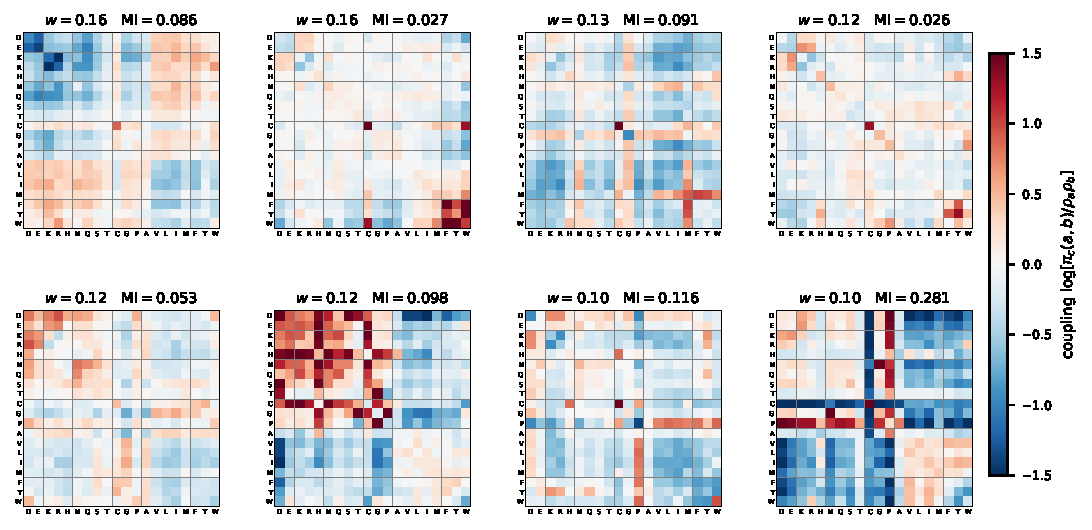
\includegraphics[width=\textwidth]{mixture_components_K8.pdf}
\caption{\textbf{The eight \Metrop-mixture coupling classes ($K{=}8$).} Each panel is
one fitted interaction class's coupling $\log[\pi_c(a,b)/\rho_a\rho_b]$ over the $400$
amino-acid pairs (red favored, blue disfavored; $\rho$ is the class marginal). Residues are ordered by group (acidic\,$|$\,basic\,$|$\,polar\,$|$\,special\,$|$\,aliphatic\,$|$\,aromatic).
Panels are sorted by mixture weight $w$ and annotated with the stationary mutual information
$\mathrm{MI}(\pi_c)$. The classes carry coherent but \emph{different} couplings---acid--base
complementarity (the off-diagonal acidic/basic blocks) in some, aliphatic assortativity (the
\texttt{AVLIM} block) in others---so pooling them into one shared chain averages
opposite-sign couplings down to the $0.026$-nat residual (\Cref{tab:pairfit}). Per-class
fitting keeps each coupling intact.}
\label{fig:components}

{\footnotesize\itshape Alt text: Eight heat-map panels, one per fitted interaction class, each covering the 400 ordered amino-acid pairs with red for favored and blue for disfavored pairs. Residues are grouped along both axes, and the panels are ordered by mixture weight.}
\end{figure}

\begin{table}[t]
\caption{Biophysical coupling in trRosetta per-contact tensors. Each axis's ``pooled'' pair covariation decomposes into ``within''-class and ``between''-classes contributions. All values are standardized to the pooled marginal (unit property
variance). ``Strength'' is the mean per-class $|\mathrm{Cov}_c|$.
``Per-class signs'' reports whether the within-class covariance is positive ($\texttt{+}$), negative ($\texttt{-}$), or near zero ($\texttt{0}$).
Charge is a weaker axis than hydropathy or volume, but it is
the only one whose within-class coupling survives pooling. This is due to
its largely consistent sign (mostly complementary); hydropathy and volume flip signs across classes and cancel.}
\label{tab:axes}
\centering
%\footnotesize
\setlength{\tabcolsep}{6pt}
\begin{tabular}{lrrrrl}
\toprule
Axis & Strength & Within (survives) & Between (comp.) & Pooled & Per-class signs\\
\midrule
Charge      & $0.10$ & $-0.096$ & $+0.014$ & $-0.082$ & \texttt{-{-}-{-}-+-{-}}\\
Hydropathy  & $0.14$ & $-0.013$ & $+0.198$ & $+0.185$ & \texttt{-0++-+-+}\\
Volume      & $0.12$ & $-0.048$ & $+0.118$ & $+0.070$ & \texttt{-+-+-+-+}\\
Aromatic    & $0.05$ & $+0.014$ & $+0.014$ & $+0.028$ & \texttt{-+0+-+-{-}}\\
\bottomrule
\end{tabular}
\end{table}

% =============================================================

% =============================================================
\subsection{Accuracy and stability of the path ELBO}
\label{sec:elboresults}
% =============================================================

\begin{figure}[t]
\centering
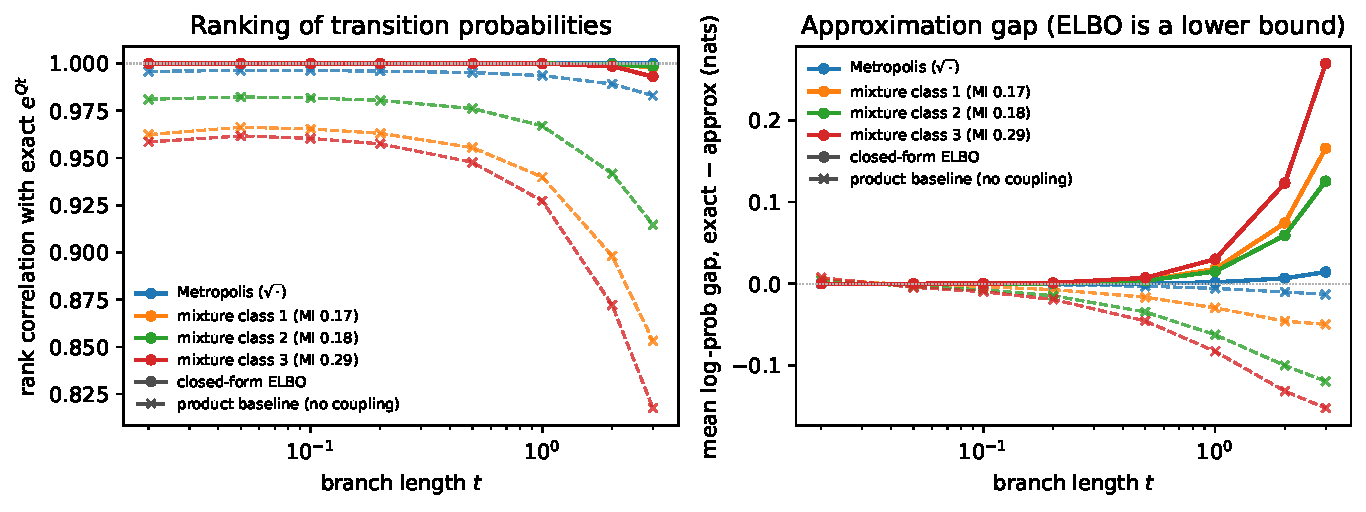
\includegraphics[width=0.78\textwidth]{figures/elbo_vs_expm_combined_legend.pdf}
\caption{\textbf{The path ELBO tracks the exact matrix exponential.} \eqref{eq:pathelbo}
for coupled pairs, where it is exactly closed-form, against exact $[e^{tW}]$ over branch
length $t$, for the \Metrop\ chain and the three strongest-coupled mixture components.
\emph{Left:} global Spearman between ELBO and exact log-transition entries (solid) stays
$\approx1$, well above the coupling-free product baseline $\prod_s[e^{tR}]_{a_sb_s}$ (dashed).
\emph{Right:} mean gap exact$-$approx; the ELBO is a lower bound near zero for
$t\lesssim1$, growing at long branches and strong coupling, while the baseline is not a
bound.}
\label{fig:elbovsexpm}

{\footnotesize\itshape Alt text: Two line plots against branch length. The left plot shows the rank correlation between the ELBO and the exact matrix exponential, with the coupling-free baseline below it; the right plot shows the mean gap between exact and approximate values.}
\end{figure}

The bound is a faithful surrogate for the exact coupled matrix exponential
(\Cref{fig:elbovsexpm}): its mean gap stays close to zero for $t\lesssim1$, and it
preserves the exact transition-probability ranking (global Spearman $\ge0.998$),
consistently above the coupling-free product baseline and by the largest margin at long
branches. Against the mean field of Cohn et al.~\citep{cohn2010} on the same pairs, our
implementation of their ODE system fails to converge on $30$--$40\%$ of pairs at short
branches, and on $\approx41\%$ of the converged ones the returned value exceeds the exact
log-likelihood; their bound is valid by construction, so these are integration errors in
the endpoint boundary layer. Their solver is also $\sim100\times$ slower.


%\paragraph{Stability against the Cohn mean field.} Compared directly to the
%endpoint-conditioned mean field of Cohn et al.~\citep{cohn2010} that it warm-starts
%(\Cref{sec:potts}), the closed form is the more dependable object
%(\Cref{fig:cohngap}): the path ELBO and its single-midpoint refinement are certified
%lower bounds, near-exact for $t\lesssim1$ and tighter still with the midpoint, while the
%full Cohn mean field---whose rate integral has an endpoint singularity---fails to
%converge on up to $30$--$40\%$ of pairs at short branches and, where it does converge,
%violates the bound on $\approx41\%$ of them. It matches Cohn's tightness without the
%ODE stiffness or bound violations, at whole-matrix rather than per-pair-ODE cost.

%\begin{figure}[t]
%\centering
%\includegraphics[width=\textwidth]{cohn_gap.pdf}
%\caption{\textbf{The closed-form ELBO is stable where the Cohn mean field is not.} Mean
%per-pair bound gap (exact $\log[e^{tW}]_{xy}$ minus approximation, nats) versus branch
%length $t$, for the two strongest-coupled \Metrop-mixture classes (stationary mutual
%information $0.16$ and $0.29$), each over $4{,}000$ importance-sampled endpoint pairs per
%branch length (full-$\psi$ Cohn over its converged subset, $\le\!92$ pairs). Curves: the
%closed-form path ELBO \eqref{eq:pathelbo}; its single-midpoint refinement (one interior
%variational node per branch---the first step of the mesh refinement of \Cref{sec:potts});
%and the Cohn mean field with and without the neighbor back-reaction $\psi$ of
%\eqref{eq:girsanov}. All four are lower bounds, so a gap $\ge0$ is required. The gray step
%(right axis) is the fraction of full-$\psi$ Cohn solves that fail to converge within a
%$16{,}384$-step ODE budget; it peaks at short branches, where the endpoint singularity of
%the Cohn rate integral is strongest. Full-$\psi$ Cohn additionally violates the bound
%(gap $<0$) at long branches, on $\approx41\%$ of converged pairs pooled across classes and
%$t$; the closed forms never do. Error bars: gap $\pm1$ SE of the mean; gray band $\pm1$ SE
%(binomial).}
%\label{fig:cohngap}
%\end{figure}

%%% I think this is the only section to drop; re: "Honestly we could probably safely
%%%   drop the product-of-trees stuff. It doesn't add much"
%Combining the closed-form ELBO above with the product-of-trees variational fit of
%Jojic et al.~\citep{JojicEtAl2004PhyloHMM} gives a method that jointly fits the Potts
%coupling and reconstructs ancestral sequences.
%the same E-step that fits $H$ keeps a
%full along-branch law per site, so it returns the posterior residue distribution at
%every internal node and coevolution-aware ancestral reconstruction is a byproduct.
%We implemented this; it works, but on protein families it returns essentially the same
%reconstructions as independent-site ASR, concordant with prior
%reports~\citep{MunizTrejo2025,ZeinatyEtAl2026ASR}. This matches our other findings in
%tone: amino-acid coupling is a minor effect in protein phylogenetics. The algorithm,
%the phylogenetic fixed-bridge Potts ELBO, is given in the supplementary appendix.



%% =============================================================
%\section{Combining coevolution with indels: the TKF--DP}
%\label{sec:tkfdp}
%% =============================================================
%
%The coupled substitution model supplies the substitution side of an indel
%model. Run TKF92 with indel parameters $(\lambda,\mu,r)$; deal each surviving
%residue, at birth, a key class $z_s$ from the stick-breaking weights of a
%Dirichlet process with concentration $\alpha_z$, so on $L$ sites the induced
%partition is Ewens~\citep{ewens1972,aldous1985} and residues sharing a table are
%coupling partners, with coevolution mediated by a ``shared field'' common to each table.
%This is the TKF Dirichlet process (TKF--DP): TKF92 with site-independence relaxed via de Finetti.
%
%\paragraph{Stationarity implies marginal-consistency.} For a coupled cluster $C$ with joint stationary
%$\pi_C$, the augmented substitution-plus-indel process is reversible at a
%deletion exactly when
%$\sum_{x_s}\pi_C(x_C)=\pi_{C\setminus s}(x_{C\setminus s})$ for every $s\in C$,
%so a residue joining a table draws from the conditional
%$\pi_C(x_s\mid x_{C\setminus s})$ and its later deletion is exact
%marginalization.
%%Iterated to any observed subset this is the projective
%%Kolmogorov condition. When it holds, the substitution factor detaches from the
%%indel bookkeeping and the alignment marginal is exactly plain TKF92's; when it
%%fails, deleting a covarying partner shifts the survivors' composition and the
%%alignment likelihood picks up a spurious dependence on the coupling. A raw
%%pairwise Potts joint violates \Cref{eq:consistency}, which is why the pair
%%Potts model needs the Sinkhorn repair of \Cref{sec:pair}; the shared field
%%satisfies it by construction, because the members are conditionally independent
%%draws from field-indexed stationaries.
%
%\paragraph{Lumpability confers indifference to ghosts.}
%In order to compute cluster likelihoods under the \TKFDP, we need to account for the possibility of transiently inserted lineages temporarily joining the cluster.
%This requires that the cluster likelihood is lumpable, surviving projection to the observed members.
%This is the motivation for having the coevolution be driven by a latent time-evolving variable associated with the site;
%the observed residues merely reflect the state of this variable.
%This further ensures marginal-consistency, as introduced in the previous paragraph.
%As a practical accommodation, if we limit clusters to two members, we can use any of the models from \Cref{sec:paircompare}.
%
%\paragraph{Alignment: the infinite pair HMM.} The generalization of the TKF92 Pair HMM to the \TKFDP\ is
%an \emph{infinite Pair HMM}~\citep{BealGhahramaniRasmussen2001} whose match states track the Ewens partition.
%We sample the joint posterior over alignments and couplings by MCMC, precomputing partial Forward matrices
%for efficient resampling of alignments between coupling pins.
%
%On the held-out Laminin EGF-like family (\Pfam\ \texttt{PF00053}) the coupled
%sampler recovers the canonical disulfide pattern from sequence alone: the eight
%conserved cysteines generate $28$ candidate Cys--Cys column pairs, and all $28$
%fall within the top $50$ column-pair posteriors, with mean Cys--Cys posterior
%$0.087$ against $0.004$ background, about $22$ times enriched
%(\Cref{fig:pf00053}). These are exactly the coevolving, indel-punctuated
%interactions that a fixed-graph alignment-conditioned Potts model is least
%equipped to recover, because the couplings and the gaps arrive together.
%Using the pairwise posteriors for multiple alignment yields improvements over plain TKF92 in sum-of-pairs (SP) and total-column (TC) accuracy
%(\Cref{tab:aln}).
%The improvement is very slight, perhaps due to the weak coupling signal in pairwise alignments.
%
%\begin{figure}[t]
%\centering
%\includegraphics[width=0.78\textwidth]{holmes_msa_triangle_PF00053_K8.pdf}
%\caption{\textbf{Coupled column-pair posterior on held-out \texttt{PF00053}.}
%All $28$ candidate Cys--Cys pairs fall in the top $50$ posteriors; the non-Cys
%top arcs cluster on the cb-EGF Ca$^{2+}$ pocket and conserved $\beta$-hairpin
%turns.}
%\label{fig:pf00053}
%\end{figure}
%
%\begin{table}[t]
%\caption{Pairwise-alignment accuracy on BAliBASE \texttt{bali3pdbm} ($L{<}150$
%subset, $22$ families / $187$ sequence pairs). For the pair-HMM models (top
%block) the MSA is assembled by feeding pairwise match posteriors into
%FSA~\citep{BradleyEtAl2009}; $F_1$, SP and TC are standard accuracy metrics. CherryML ($C{=}20$) is a $20$-class site mixture fitted by
%CherryML~\citep{Prillo2023CherryML}. MAFFT~\citep{Katoh2013} and
%MUSCLE~\citep{Edgar2004} are shown for reference.}
%\label{tab:aln}
%\centering
%\footnotesize
%\setlength{\tabcolsep}{6pt}
%\begin{tabular}{lccc}
%\toprule
%Method & MSA $F_1$ & SP & TC\\
%\midrule
%TKF92                            & 0.514 & 0.724 & 0.631\\
%TKF92 ($K_c{=}20$)               & 0.515 & 0.732 & 0.637\\
%CherryML ($C{=}20$)              & 0.515 & 0.723 & 0.629\\
%Coupled $K_c{=}8$                & 0.513 & 0.730 & 0.640\\
%\midrule
%MAFFT (FFT-NS-2)                 & 0.509 & 0.691 & 0.558\\
%MUSCLE (default)                 & 0.512 & 0.760 & 0.662\\
%\bottomrule
%\end{tabular}
%\end{table}

% =============================================================
\section{Discussion}
\label{sec:discussion}
% =============================================================

Symmetry is central to molecular evolution: the invariants (reversibility,
exchangeability) and the equivariants (lumpability) of a coupled substitution process
inform the design of a coevolutionary model. EM and variational Bayes can help.
Locally-correlated rate heterogeneity, needed by models that partition by domain or
secondary structure~\citep{LargeHolmes2026,ThorneGoldmanJones96,Yang1995}, is a natural
complement to this work.

% Do NOT include this section in the anonymized submission, only in the final paper. You can use the \texttt{ack} environment provided in the style file to automatically hide this section in the anonymized submission.
%\begin{ack}
%We thank Debora Marks, Yun Song, and Sebastian Prillo for helpful discussions. Selected mathematical
%derivations and exposition were generated by Anthropic and OpenAI products
%under the supervision of the human authors. The work was funded
%by NIH grants HG004483, GM080203, and HG013117.
%\end{ack}

%% References follow the acknowledgments and do not count towards the page
%% limit.  natbib+plainnat sets the unnumbered "References" heading itself.
%% The .bib file lives in this directory.
\label{endofbody}

% =============================================================
\section*{Data availability}
% =============================================================

This study generated no new sequence or structural data. The coupled
substitution count tensors were assembled from the publicly available
trRosetta training set of structures and alignments \citep{Yang2020trRosetta}.
Source code for the models, the count-tensor pipeline and the ELBO, together
with the fitted parameters and the scripts that regenerate every table and
figure in this paper, is available at
\url{https://github.com/evoldoers/tkfdp}.

% =============================================================
\section*{Acknowledgements}
% =============================================================

We thank Debora Marks, Yun Song, and Sebastian Prillo for helpful discussions.
Some of the mathematical derivations, exposition and code in this work were
drafted with the assistance of large language models (Anthropic's Claude and
OpenAI's ChatGPT) and were then checked and edited by the authors, who take full
responsibility for the content.

\subsection*{Funding}

This work was supported by the National Institutes of Health
(HG004483, GM080203, HG013117).

% =============================================================
\section*{Conflict of interest}
% =============================================================

The authors declare no conflict of interest.

\newpage
\bibliographystyle{abbrvnat}
\bibliography{refs}

\end{document}
